% Options for packages loaded elsewhere
\PassOptionsToPackage{unicode}{hyperref}
\PassOptionsToPackage{hyphens}{url}
%
\documentclass[
]{article}
\usepackage{amsmath,amssymb}
\usepackage{lmodern}
\usepackage{iftex}
\ifPDFTeX
  \usepackage[T1]{fontenc}
  \usepackage[utf8]{inputenc}
  \usepackage{textcomp} % provide euro and other symbols
\else % if luatex or xetex
  \usepackage{unicode-math}
  \defaultfontfeatures{Scale=MatchLowercase}
  \defaultfontfeatures[\rmfamily]{Ligatures=TeX,Scale=1}
\fi
% Use upquote if available, for straight quotes in verbatim environments
\IfFileExists{upquote.sty}{\usepackage{upquote}}{}
\IfFileExists{microtype.sty}{% use microtype if available
  \usepackage[]{microtype}
  \UseMicrotypeSet[protrusion]{basicmath} % disable protrusion for tt fonts
}{}
\makeatletter
\@ifundefined{KOMAClassName}{% if non-KOMA class
  \IfFileExists{parskip.sty}{%
    \usepackage{parskip}
  }{% else
    \setlength{\parindent}{0pt}
    \setlength{\parskip}{6pt plus 2pt minus 1pt}}
}{% if KOMA class
  \KOMAoptions{parskip=half}}
\makeatother
\usepackage{xcolor}
\usepackage[margin=1in]{geometry}
\usepackage{color}
\usepackage{fancyvrb}
\newcommand{\VerbBar}{|}
\newcommand{\VERB}{\Verb[commandchars=\\\{\}]}
\DefineVerbatimEnvironment{Highlighting}{Verbatim}{commandchars=\\\{\}}
% Add ',fontsize=\small' for more characters per line
\usepackage{framed}
\definecolor{shadecolor}{RGB}{248,248,248}
\newenvironment{Shaded}{\begin{snugshade}}{\end{snugshade}}
\newcommand{\AlertTok}[1]{\textcolor[rgb]{0.94,0.16,0.16}{#1}}
\newcommand{\AnnotationTok}[1]{\textcolor[rgb]{0.56,0.35,0.01}{\textbf{\textit{#1}}}}
\newcommand{\AttributeTok}[1]{\textcolor[rgb]{0.77,0.63,0.00}{#1}}
\newcommand{\BaseNTok}[1]{\textcolor[rgb]{0.00,0.00,0.81}{#1}}
\newcommand{\BuiltInTok}[1]{#1}
\newcommand{\CharTok}[1]{\textcolor[rgb]{0.31,0.60,0.02}{#1}}
\newcommand{\CommentTok}[1]{\textcolor[rgb]{0.56,0.35,0.01}{\textit{#1}}}
\newcommand{\CommentVarTok}[1]{\textcolor[rgb]{0.56,0.35,0.01}{\textbf{\textit{#1}}}}
\newcommand{\ConstantTok}[1]{\textcolor[rgb]{0.00,0.00,0.00}{#1}}
\newcommand{\ControlFlowTok}[1]{\textcolor[rgb]{0.13,0.29,0.53}{\textbf{#1}}}
\newcommand{\DataTypeTok}[1]{\textcolor[rgb]{0.13,0.29,0.53}{#1}}
\newcommand{\DecValTok}[1]{\textcolor[rgb]{0.00,0.00,0.81}{#1}}
\newcommand{\DocumentationTok}[1]{\textcolor[rgb]{0.56,0.35,0.01}{\textbf{\textit{#1}}}}
\newcommand{\ErrorTok}[1]{\textcolor[rgb]{0.64,0.00,0.00}{\textbf{#1}}}
\newcommand{\ExtensionTok}[1]{#1}
\newcommand{\FloatTok}[1]{\textcolor[rgb]{0.00,0.00,0.81}{#1}}
\newcommand{\FunctionTok}[1]{\textcolor[rgb]{0.00,0.00,0.00}{#1}}
\newcommand{\ImportTok}[1]{#1}
\newcommand{\InformationTok}[1]{\textcolor[rgb]{0.56,0.35,0.01}{\textbf{\textit{#1}}}}
\newcommand{\KeywordTok}[1]{\textcolor[rgb]{0.13,0.29,0.53}{\textbf{#1}}}
\newcommand{\NormalTok}[1]{#1}
\newcommand{\OperatorTok}[1]{\textcolor[rgb]{0.81,0.36,0.00}{\textbf{#1}}}
\newcommand{\OtherTok}[1]{\textcolor[rgb]{0.56,0.35,0.01}{#1}}
\newcommand{\PreprocessorTok}[1]{\textcolor[rgb]{0.56,0.35,0.01}{\textit{#1}}}
\newcommand{\RegionMarkerTok}[1]{#1}
\newcommand{\SpecialCharTok}[1]{\textcolor[rgb]{0.00,0.00,0.00}{#1}}
\newcommand{\SpecialStringTok}[1]{\textcolor[rgb]{0.31,0.60,0.02}{#1}}
\newcommand{\StringTok}[1]{\textcolor[rgb]{0.31,0.60,0.02}{#1}}
\newcommand{\VariableTok}[1]{\textcolor[rgb]{0.00,0.00,0.00}{#1}}
\newcommand{\VerbatimStringTok}[1]{\textcolor[rgb]{0.31,0.60,0.02}{#1}}
\newcommand{\WarningTok}[1]{\textcolor[rgb]{0.56,0.35,0.01}{\textbf{\textit{#1}}}}
\usepackage{graphicx}
\makeatletter
\def\maxwidth{\ifdim\Gin@nat@width>\linewidth\linewidth\else\Gin@nat@width\fi}
\def\maxheight{\ifdim\Gin@nat@height>\textheight\textheight\else\Gin@nat@height\fi}
\makeatother
% Scale images if necessary, so that they will not overflow the page
% margins by default, and it is still possible to overwrite the defaults
% using explicit options in \includegraphics[width, height, ...]{}
\setkeys{Gin}{width=\maxwidth,height=\maxheight,keepaspectratio}
% Set default figure placement to htbp
\makeatletter
\def\fps@figure{htbp}
\makeatother
\setlength{\emergencystretch}{3em} % prevent overfull lines
\providecommand{\tightlist}{%
  \setlength{\itemsep}{0pt}\setlength{\parskip}{0pt}}
\setcounter{secnumdepth}{-\maxdimen} % remove section numbering
\usepackage{booktabs}
\usepackage{float}
\usepackage{array}
\usepackage{multirow}
\floatplacement{figure}{H}
\usepackage{booktabs}
\usepackage{longtable}
\usepackage{array}
\usepackage{multirow}
\usepackage{wrapfig}
\usepackage{float}
\usepackage{colortbl}
\usepackage{pdflscape}
\usepackage{tabu}
\usepackage{threeparttable}
\usepackage{threeparttablex}
\usepackage[normalem]{ulem}
\usepackage{makecell}
\usepackage{xcolor}
\ifLuaTeX
  \usepackage{selnolig}  % disable illegal ligatures
\fi
\IfFileExists{bookmark.sty}{\usepackage{bookmark}}{\usepackage{hyperref}}
\IfFileExists{xurl.sty}{\usepackage{xurl}}{} % add URL line breaks if available
\urlstyle{same} % disable monospaced font for URLs
\hypersetup{
  pdftitle={rjdmarkdown with PDF output},
  hidelinks,
  pdfcreator={LaTeX via pandoc}}

\title{rjdmarkdown with PDF output}
\author{}
\date{\vspace{-2.5em}}

\begin{document}
\maketitle

The functions developped in \texttt{rjdmarkdown} are:

\begin{itemize}
\tightlist
\item
  \texttt{print\_preprocessing()} for the pre-processing model;\\
\item
  \texttt{print\_decomposition()} for the decomposition;\\
\item
  \texttt{print\_diagnostics()} to print diagnostics tests on the
  quality of the seasonal adjustment.
\end{itemize}

The result is different between X-13ARIMA and TRAMO-SEATS models.

\begin{Shaded}
\begin{Highlighting}[]
\FunctionTok{library}\NormalTok{(rjdmarkdown)}
\FunctionTok{library}\NormalTok{(RJDemetra)}
\NormalTok{sa\_x13 }\OtherTok{\textless{}{-}} \FunctionTok{x13}\NormalTok{(ipi\_c\_eu[, }\StringTok{"FR"}\NormalTok{])}
\NormalTok{sa\_ts }\OtherTok{\textless{}{-}} \FunctionTok{tramoseats}\NormalTok{(ipi\_c\_eu[, }\StringTok{"FR"}\NormalTok{])}
\end{Highlighting}
\end{Shaded}

\hypertarget{x-13-arima-model}{%
\section{X-13-ARIMA model}\label{x-13-arima-model}}

\begin{Shaded}
\begin{Highlighting}[]
\FunctionTok{print\_preprocessing}\NormalTok{(sa\_x13)}
\end{Highlighting}
\end{Shaded}

\underline{\textbf{Pre-processing (RegArima)}}

\underline{\textbf{Summary}}

372 observations

Trading days effect (7 variables)

Easter {[}1{]} detected

4 detected outliers

\underline{\textbf{Likelihood statistics}}

Number of effective observations = 359

Number of estimated parameters = 17

Loglikelihood = -799.084, AICc = 1633.964, BICc = 1.855

Standard error of the regression (ML estimate) = 2.218

\underline{\textbf{ARIMA model}}

\begin{table}[H]
\centering
\caption{\label{tab:unnamed-chunk-3}ARIMA coefficients}
\centering
\begin{tabular}[t]{lccccc}
\toprule
  & Coefficients & Std. Error & T-stat & $\mathbb P (> \lvert t \rvert)$ & \\
\midrule
Phi(1) & 0.000 & 0.108 & 0.003 & 0.998 & \\
Phi(2) & 0.169 & 0.074 & 2.278 & 0.023 & *\\
Theta(1) & -0.549 & 0.102 & -5.396 & 0.000 & ***\\
BTheta(1) & -0.666 & 0.042 & -15.775 & 0.000 & ***\\
\bottomrule
\multicolumn{6}{l}{\rule{0pt}{1em}\textbf{Signif. codes: }0 `***' 0.001 `**' 0.01 `*' 0.05 `.' 0.1 ` ' 1}\\
\multicolumn{6}{l}{\rule{0pt}{1em}ARIMA (2,1,1)(0,1,1)}\\
\end{tabular}
\end{table}

\underline{\textbf{Regression model}}

\begin{table}[H]
\centering
\caption{\label{tab:unnamed-chunk-3}Regression coefficientss}
\centering
\begin{tabular}[t]{lccccc}
\toprule
  & Coefficients & Std. Error & T-stat & $\mathbb P (> \lvert t \rvert)$ & \\
\midrule
Monday & 0.559 & 0.228 & 2.453 & 0.015 & *\\
Tuesday & 0.882 & 0.228 & 3.864 & 0.000 & ***\\
Wednesday & 1.040 & 0.229 & 4.535 & 0.000 & ***\\
Thursday & 0.049 & 0.229 & 0.215 & 0.830 & \\
Friday & 0.911 & 0.230 & 3.964 & 0.000 & ***\\
\addlinespace
Saturday & -1.578 & 0.228 & -6.927 & 0.000 & ***\\
Leap year & 2.154 & 0.705 & 3.054 & 0.002 & **\\
Easter [1] & -2.380 & 0.454 & -5.242 & 0.000 & ***\\
TC (4-2020) & -35.592 & 2.173 & -16.377 & 0.000 & ***\\
AO (3-2020) & -20.890 & 2.180 & -9.582 & 0.000 & ***\\
\addlinespace
AO (5-2011) & 13.499 & 1.857 & 7.269 & 0.000 & ***\\
LS (11-2008) & -12.549 & 1.636 & -7.673 & 0.000 & ***\\
\bottomrule
\multicolumn{6}{l}{\rule{0pt}{1em}\textbf{Signif. codes: }0 `***' 0.001 `**' 0.01 `*' 0.05 `.' 0.1 ` ' 1}\\
\end{tabular}
\end{table}

\begin{Shaded}
\begin{Highlighting}[]
\FunctionTok{print\_decomposition}\NormalTok{(sa\_x13, }\AttributeTok{caption =} \ConstantTok{NULL}\NormalTok{)}
\end{Highlighting}
\end{Shaded}

\underline{\textbf{Decomposition (X-11)}}

Mode: additive

\begin{figure}
\centering
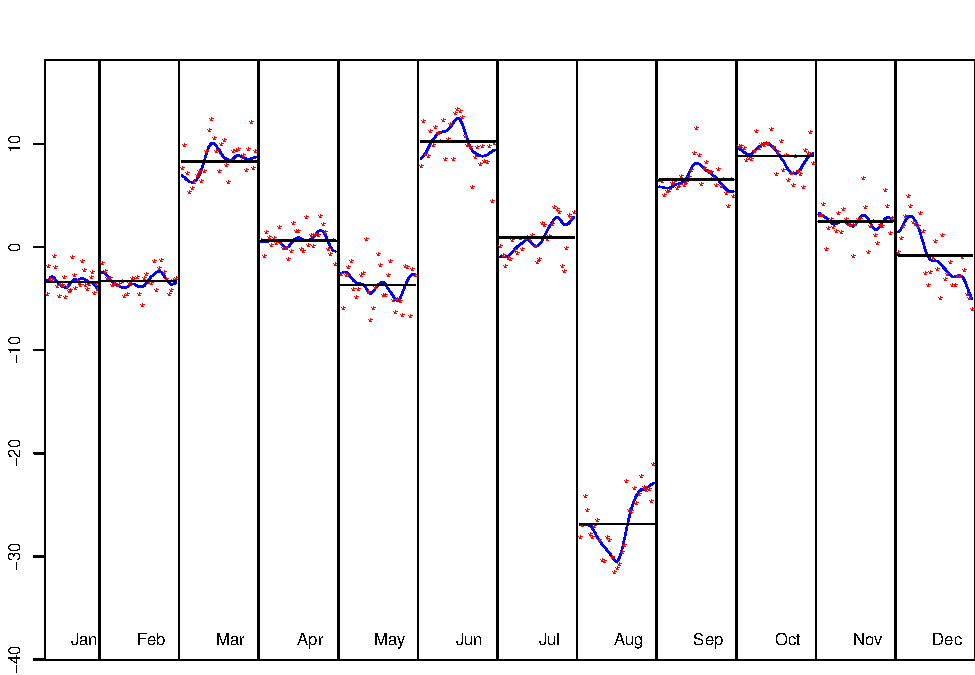
\includegraphics{/home/runner/work/rjdmarkdown/rjdmarkdown/docs/articles/rjdmarkdown-pdf_files/figure-latex/unnamed-chunk-3-1.pdf}
\caption{S-I Ratio}
\end{figure}

\begin{table}[H]
\centering
\caption{\label{tab:unnamed-chunk-3}M-statistics}
\centering
\begin{tabular}[t]{lc>{\raggedright\arraybackslash}p{0.7\textwidth}}
\toprule
  & Value & Description\\
\midrule
M-1 & 0.163 & The relative contribution of the irregular over three months span\\
M-2 & 0.089 & The relative contribution of the irregular component to the stationary portion of the variance\\
M-3 & 1.181 & The amount of period to period change in the irregular component as compared to the amount of period to period change in the trend\\
M-4 & 0.558 & The amount of autocorrelation in the irregular as described by the average duration of run\\
M-5 & 1.020 & The number of periods it takes the change in the trend to surpass the amount of change in the irregular\\
\addlinespace
M-6 & 0.090 & The amount of year to year change in the irregular as compared to the amount of year to year change in the seasonal\\
M-7 & 0.083 & The amount of moving seasonality present relative to the amount of stable seasonality\\
M-8 & 0.244 & The size of the fluctuations in the seasonal component throughout the whole series\\
M-9 & 0.062 & The average linear movement in the seasonal component throughout the whole series\\
M-10 & 0.272 & The size of the fluctuations in the seasonal component in the recent years\\
\addlinespace
M-11 & 0.256 & The average linear movement in the seasonal component in the recent years\\
Q & 0.368 & \\
Q-M2 & 0.402 & \\
\bottomrule
\multicolumn{3}{l}{\rule{0pt}{1em}\textbf{Final filters}: M3x5, Henderson-13 terms}\\
\end{tabular}
\end{table}

\begin{table}[H]
\centering
\caption{\label{tab:unnamed-chunk-3}Relative contribution of the components to the stationary portion of the variance in the original series, after the removal of the long term trend}
\centering
\begin{tabular}[t]{lc}
\toprule
  & Component\\
\midrule
Cycle & 2.251\\
Seasonal & 59.750\\
Irregular & 1.067\\
TD \& Hol. & 2.610\\
Others & 33.718\\
\addlinespace
Total & 99.395\\
\bottomrule
\end{tabular}
\end{table}

\begin{Shaded}
\begin{Highlighting}[]
\FunctionTok{print\_diagnostics}\NormalTok{(sa\_x13)}
\end{Highlighting}
\end{Shaded}

\begin{table}[H]
\centering
\caption{\label{tab:unnamed-chunk-3}Diagnostics tests}
\centering
\begin{tabular}[t]{l|c|c}
\hline
  & $\mathbb P (> \lvert t \rvert)$ & \\
\hline
mean & 0.899 & \\
\hline
skewness & 0.880 & \\
\hline
kurtosis & 0.034 & *\\
\hline
ljung box & 0.000 & ***\\
\hline
ljung box (residuals at seasonal lags) & 0.212 & \\
\hline
ljung box (squared residuals) & 0.024 & *\\
\hline
qs test on sa & 0.985 & \\
\hline
qs test on i & 0.865 & \\
\hline
f-test on sa (seasonal dummies) & 0.958 & \\
\hline
f-test on i (seasonal dummies) & 0.893 & \\
\hline
Residual seasonality (entire series) & 0.876 & \\
\hline
Residual seasonality (last 3 years) & 0.906 & \\
\hline
f-test on sa (td) & 0.987 & \\
\hline
f-test on i (td) & 0.993 & \\
\hline
\multicolumn{3}{l}{\rule{0pt}{1em}\textbf{Signif. codes: }0 `***' 0.001 `**' 0.01 `*' 0.05 `.' 0.1 ` ' 1}\\
\end{tabular}
\end{table}

\hypertarget{tramo-seats-model}{%
\section{TRAMO-SEATS model}\label{tramo-seats-model}}

Some others graphics can also be added with the
\href{https://aqlt.github.io/ggdemetra/}{\texttt{ggdemetra}} package,
for example to add the seasonally adjusted series and its forecasts:

\begin{Shaded}
\begin{Highlighting}[]
\FunctionTok{library}\NormalTok{(ggdemetra)}
\FunctionTok{ggplot}\NormalTok{(}\AttributeTok{data =}\NormalTok{ ipi\_c\_eu\_df, }\AttributeTok{mapping =} \FunctionTok{aes}\NormalTok{(}\AttributeTok{x =}\NormalTok{ date, }\AttributeTok{y =}\NormalTok{ FR)) }\SpecialCharTok{+}
    \FunctionTok{geom\_line}\NormalTok{() }\SpecialCharTok{+}
    \FunctionTok{labs}\NormalTok{(}\AttributeTok{title =} \ConstantTok{NULL}\NormalTok{,}
         \AttributeTok{x =} \ConstantTok{NULL}\NormalTok{, }\AttributeTok{y =} \ConstantTok{NULL}\NormalTok{) }\SpecialCharTok{+}
    \FunctionTok{geom\_sa}\NormalTok{(}\AttributeTok{component =} \StringTok{"y\_f"}\NormalTok{, }\AttributeTok{linetype =} \DecValTok{2}\NormalTok{,}
            \AttributeTok{frequency =} \DecValTok{12}\NormalTok{, }\AttributeTok{method =} \StringTok{"tramoseats"}\NormalTok{) }\SpecialCharTok{+} 
    \FunctionTok{geom\_sa}\NormalTok{(}\AttributeTok{component =} \StringTok{"sa"}\NormalTok{, }\AttributeTok{color =} \StringTok{"red"}\NormalTok{) }\SpecialCharTok{+}
    \FunctionTok{geom\_sa}\NormalTok{(}\AttributeTok{component =} \StringTok{"sa\_f"}\NormalTok{, }\AttributeTok{color =} \StringTok{"red"}\NormalTok{, }\AttributeTok{linetype =} \DecValTok{2}\NormalTok{)}
\end{Highlighting}
\end{Shaded}

\begin{figure}
\centering
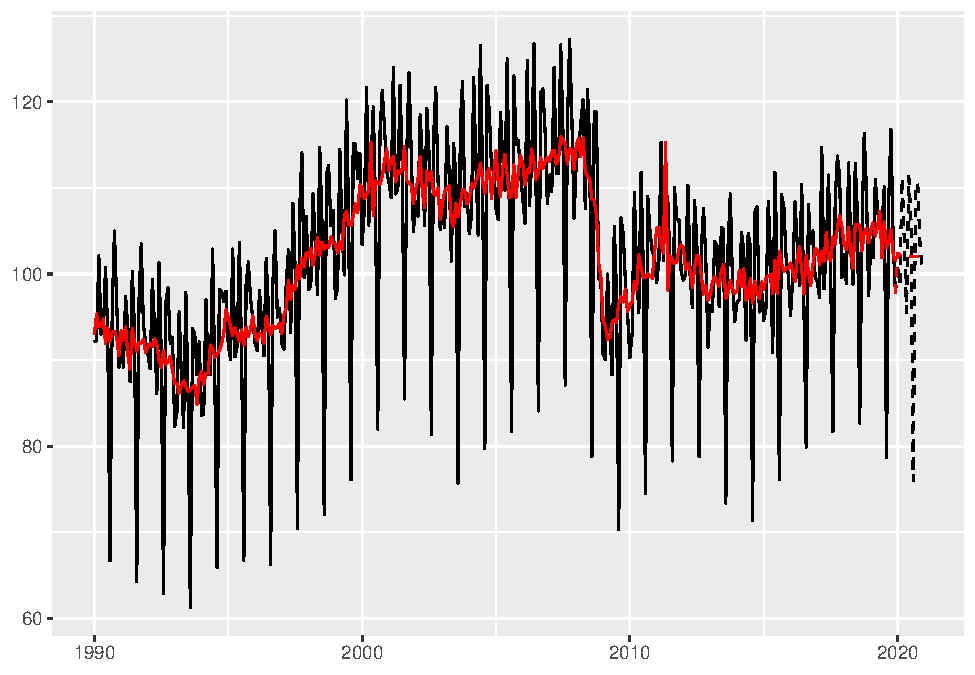
\includegraphics{/home/runner/work/rjdmarkdown/rjdmarkdown/docs/articles/rjdmarkdown-pdf_files/figure-latex/unnamed-chunk-4-1.pdf}
\caption{Seasonal adjustment of the French industrial production index}
\end{figure}

\begin{Shaded}
\begin{Highlighting}[]
\FunctionTok{print\_preprocessing}\NormalTok{(sa\_ts)}
\end{Highlighting}
\end{Shaded}

\underline{\textbf{Pre-processing (Tramo)}}

\underline{\textbf{Summary}}

372 observations

Trading days effect (2 variables)

Easter {[}6{]} detected

4 detected outliers

\underline{\textbf{Likelihood statistics}}

Number of effective observations = 359

Number of estimated parameters = 11

Loglikelihood = -816.075, AICc = 1654.912, BICc = 1.852

Standard error of the regression (ML estimate) = 2.326

\underline{\textbf{ARIMA model}}

\begin{table}[H]
\centering
\caption{\label{tab:unnamed-chunk-4}ARIMA coefficients}
\centering
\begin{tabular}[t]{lccccc}
\toprule
  & Coefficients & Std. Error & T-stat & $\mathbb P (> \lvert t \rvert)$ & \\
\midrule
Phi(1) & 0.403 & 0.051 & 7.845 & 0.000 & ***\\
Phi(2) & 0.288 & 0.051 & 5.616 & 0.000 & ***\\
BTheta(1) & -0.664 & 0.042 & -15.865 & 0.000 & ***\\
\bottomrule
\multicolumn{6}{l}{\rule{0pt}{1em}\textbf{Signif. codes: }0 `***' 0.001 `**' 0.01 `*' 0.05 `.' 0.1 ` ' 1}\\
\multicolumn{6}{l}{\rule{0pt}{1em}ARIMA (2,1,0)(0,1,1)}\\
\end{tabular}
\end{table}

\underline{\textbf{Regression model}}

\begin{table}[H]
\centering
\caption{\label{tab:unnamed-chunk-4}Regression coefficientss}
\centering
\begin{tabular}[t]{lccccc}
\toprule
  & Coefficients & Std. Error & T-stat & $\mathbb P (> \lvert t \rvert)$ & \\
\midrule
Week days & 0.699 & 0.032 & 22.016 & 0.000 & ***\\
Leap year & 2.323 & 0.690 & 3.367 & 0.001 & ***\\
Easter [6] & -2.515 & 0.436 & -5.773 & 0.000 & ***\\
AO (5-2011) & 13.468 & 1.787 & 7.535 & 0.000 & ***\\
TC (4-2020) & -22.213 & 2.205 & -10.072 & 0.000 & ***\\
\addlinespace
TC (3-2020) & -21.039 & 2.217 & -9.492 & 0.000 & ***\\
AO (5-2000) & 6.739 & 1.794 & 3.757 & 0.000 & ***\\
\bottomrule
\multicolumn{6}{l}{\rule{0pt}{1em}\textbf{Signif. codes: }0 `***' 0.001 `**' 0.01 `*' 0.05 `.' 0.1 ` ' 1}\\
\end{tabular}
\end{table}

\begin{Shaded}
\begin{Highlighting}[]
\FunctionTok{print\_decomposition}\NormalTok{(sa\_ts, }\AttributeTok{caption =} \ConstantTok{NULL}\NormalTok{)}
\end{Highlighting}
\end{Shaded}

\underline{\textbf{Decomposition (SEATS)}}

Mode: additive

\begin{figure}
\centering
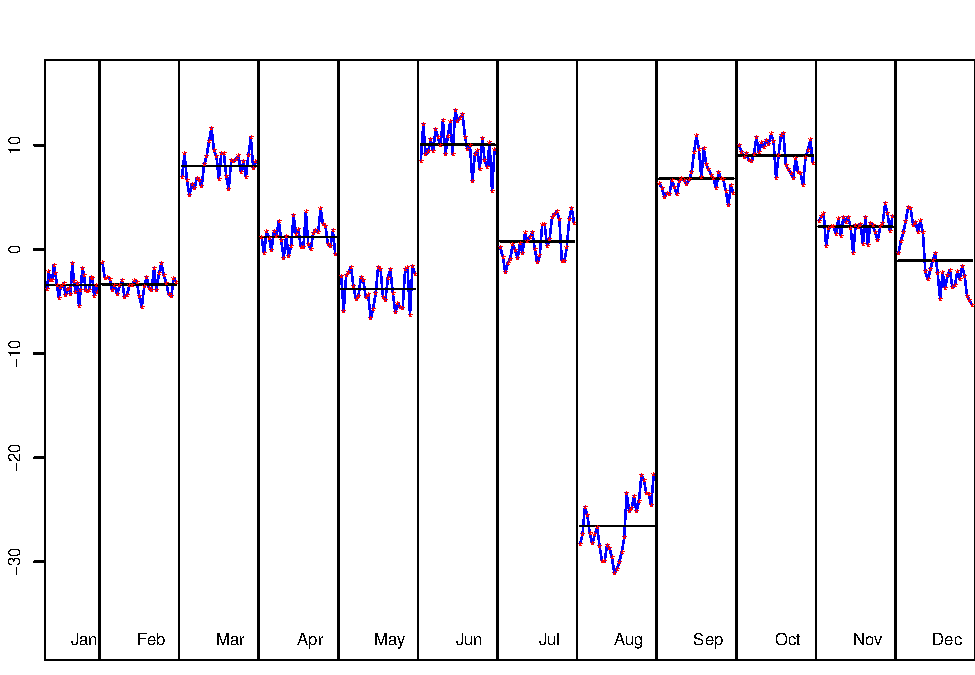
\includegraphics{/home/runner/work/rjdmarkdown/rjdmarkdown/docs/articles/rjdmarkdown-pdf_files/figure-latex/unnamed-chunk-4-2.pdf}
\caption{S-I Ratio}
\end{figure}

\textbf{Model}

AR: \(1+0.403B+0.288B^{2}\)

D: \(1-B-B^{12}+B^{13}\)

MA: \(1-0.664B^{12}\)

\textbf{SA}

AR: \(1+0.403B+0.288B^{2}\)

D: \(1-2.000B+B^{2}\)

MA: \(1-0.970B+0.006B^{2}-0.006B^{3}+0.004B^{4}\)

Innovation variance: 0.704

\textbf{Trend}

D: \(1-2.000B+B^{2}\)

MA: \(1+0.034B-0.966B^{2}\)

Innovation variance: 0.061

\textbf{Seasonal}

D: \(1+B+B^{2}+B^{3}+B^{4}+B^{5}+B^{6}+B^{7}+B^{8}+B^{9}+B^{10}+B^{11}\)

MA:
\(1+1.329B+1.106B^{2}+1.185B^{3}+1.068B^{4}+0.821B^{5}+0.632B^{6}+0.404B^{7}+0.245B^{8}+0.002B^{9}-0.056B^{10}-0.204B^{11}\)

Innovation variance: 0.043

\textbf{Transitory}

AR: \(1+0.403B+0.288B^{2}\)

MA: \(1-0.260B-0.740B^{2}\)

Innovation variance: 0.053

\textbf{Irregular}

Innovation variance: 0.203

\begin{table}[H]
\centering
\caption{\label{tab:unnamed-chunk-4}Relative contribution of the components to the stationary portion of the variance in the original series, after the removal of the long term trend}
\centering
\begin{tabular}[t]{lc}
\toprule
  & Component\\
\midrule
Cycle & 6.087\\
Seasonal & 80.528\\
Irregular & 0.965\\
TD \& Hol. & 3.590\\
Others & 8.102\\
\addlinespace
Total & 99.271\\
\bottomrule
\end{tabular}
\end{table}

\begin{Shaded}
\begin{Highlighting}[]
\FunctionTok{print\_diagnostics}\NormalTok{(sa\_ts)}
\end{Highlighting}
\end{Shaded}

\begin{table}[H]
\centering
\caption{\label{tab:unnamed-chunk-4}Diagnostics tests}
\centering
\begin{tabular}[t]{l|c|c}
\hline
  & $\mathbb P (> \lvert t \rvert)$ & \\
\hline
mean & 0.988 & \\
\hline
skewness & 0.413 & \\
\hline
kurtosis & 0.095 & .\\
\hline
ljung box & 0.010 & **\\
\hline
ljung box (residuals at seasonal lags) & 0.192 & \\
\hline
ljung box (squared residuals) & 0.000 & ***\\
\hline
qs test on sa & 1.000 & \\
\hline
qs test on i & 1.000 & \\
\hline
f-test on sa (seasonal dummies) & 1.000 & \\
\hline
f-test on i (seasonal dummies) & 1.000 & \\
\hline
Residual seasonality (entire series) & 1.000 & \\
\hline
Residual seasonality (last 3 years) & 0.974 & \\
\hline
f-test on sa (td) & 0.152 & \\
\hline
f-test on i (td) & 0.224 & \\
\hline
\multicolumn{3}{l}{\rule{0pt}{1em}\textbf{Signif. codes: }0 `***' 0.001 `**' 0.01 `*' 0.05 `.' 0.1 ` ' 1}\\
\end{tabular}
\end{table}

\hypertarget{directly-create-a-r-markdown-file}{%
\section{Directly create a R Markdown
file}\label{directly-create-a-r-markdown-file}}

A R Markdown can also directly be created and render with the
\texttt{create\_rmd} function. It can take as argument a \texttt{SA},
\texttt{jSA}, \texttt{sa\_item}, \texttt{multiprocessing} (all the
models of the \texttt{multiprocessing} are printed) or workspace object
(all the models of all the \texttt{multiprocessing} of the
\texttt{workspace} are printed).

The print of the pre-processing, decomposition and diagnostics can also
be customized with \texttt{preprocessing\_fun},
\texttt{decomposition\_fun} and \texttt{diagnostics\_fun} arguments. For
example, to reproduce the example of the previous section:

\begin{Shaded}
\begin{Highlighting}[]
\NormalTok{preprocessing\_customized }\OtherTok{\textless{}{-}} \ControlFlowTok{function}\NormalTok{(x)\{}
  \FunctionTok{library}\NormalTok{(ggdemetra)}
\NormalTok{  y }\OtherTok{\textless{}{-}} \FunctionTok{get\_ts}\NormalTok{(x)}
\NormalTok{  data\_plot }\OtherTok{\textless{}{-}} \FunctionTok{data.frame}\NormalTok{(}\AttributeTok{date =} \FunctionTok{time}\NormalTok{(y), }\AttributeTok{y =}\NormalTok{ y)}
\NormalTok{  p }\OtherTok{\textless{}{-}} \FunctionTok{ggplot}\NormalTok{(}\AttributeTok{data =}\NormalTok{ data\_plot, }\AttributeTok{mapping =} \FunctionTok{aes}\NormalTok{(}\AttributeTok{x =}\NormalTok{ date, }\AttributeTok{y =}\NormalTok{ y)) }\SpecialCharTok{+}
    \FunctionTok{geom\_line}\NormalTok{() }\SpecialCharTok{+}
    \FunctionTok{labs}\NormalTok{(}\AttributeTok{title =} \ConstantTok{NULL}\NormalTok{,}
         \AttributeTok{x =} \ConstantTok{NULL}\NormalTok{, }\AttributeTok{y =} \ConstantTok{NULL}\NormalTok{) }\SpecialCharTok{+}
    \FunctionTok{geom\_sa}\NormalTok{(}\AttributeTok{component =} \StringTok{"y\_f"}\NormalTok{, }\AttributeTok{linetype =} \DecValTok{2}\NormalTok{,}
            \AttributeTok{frequency =} \DecValTok{12}\NormalTok{, }\AttributeTok{method =} \StringTok{"tramoseats"}\NormalTok{) }\SpecialCharTok{+}
    \FunctionTok{geom\_sa}\NormalTok{(}\AttributeTok{component =} \StringTok{"sa"}\NormalTok{, }\AttributeTok{color =} \StringTok{"red"}\NormalTok{) }\SpecialCharTok{+}
    \FunctionTok{geom\_sa}\NormalTok{(}\AttributeTok{component =} \StringTok{"sa\_f"}\NormalTok{, }\AttributeTok{color =} \StringTok{"red"}\NormalTok{, }\AttributeTok{linetype =} \DecValTok{2}\NormalTok{)}
  \FunctionTok{plot}\NormalTok{(p)}
  \FunctionTok{cat}\NormalTok{(}\StringTok{"}\SpecialCharTok{\textbackslash{}n\textbackslash{}n}\StringTok{"}\NormalTok{)}
  \FunctionTok{print\_preprocessing}\NormalTok{(sa\_ts)}
\NormalTok{\}}
\NormalTok{decomposition\_customized }\OtherTok{\textless{}{-}} \ControlFlowTok{function}\NormalTok{(x)\{}
  \FunctionTok{print\_decomposition}\NormalTok{(x, }\AttributeTok{caption =} \ConstantTok{NULL}\NormalTok{)}
\NormalTok{\}}

\NormalTok{output\_file }\OtherTok{\textless{}{-}} \FunctionTok{tempfile}\NormalTok{(}\AttributeTok{fileext =} \StringTok{".Rmd"}\NormalTok{)}

\FunctionTok{create\_rmd}\NormalTok{(sa\_ts, output\_file, }\AttributeTok{output\_format =} \StringTok{"pdf\_document"}\NormalTok{,}
           \AttributeTok{preprocessing\_fun =}\NormalTok{ preprocessing\_customized,}
           \AttributeTok{decomposition\_fun =}\NormalTok{ decomposition\_customized,}
           \AttributeTok{knitr\_chunk\_opts =} \FunctionTok{list}\NormalTok{(}
             \AttributeTok{fig.pos =} \StringTok{"h"}\NormalTok{, }\AttributeTok{results =} \StringTok{"asis"}\NormalTok{, }
             \AttributeTok{fig.cap =}\FunctionTok{c}\NormalTok{(}\StringTok{"Seasonal adjustment of the French industrial production index"}\NormalTok{,}
                        \StringTok{"S{-}I Ratio"}\NormalTok{),}
             \AttributeTok{warning =} \ConstantTok{FALSE}\NormalTok{, }\AttributeTok{message =} \ConstantTok{FALSE}\NormalTok{, }\AttributeTok{echo =} \ConstantTok{FALSE}\NormalTok{)}
\NormalTok{           )}
\CommentTok{\# To open the file:}
\FunctionTok{browseURL}\NormalTok{(}\FunctionTok{sub}\NormalTok{(}\StringTok{".Rmd"}\NormalTok{,}\StringTok{".pdf"}\NormalTok{, output\_file, }\AttributeTok{fixed=} \ConstantTok{TRUE}\NormalTok{))}
\end{Highlighting}
\end{Shaded}

Several models can also be printed creating a workspace:

\begin{Shaded}
\begin{Highlighting}[]
\NormalTok{wk }\OtherTok{\textless{}{-}} \FunctionTok{new\_workspace}\NormalTok{()}
\FunctionTok{new\_multiprocessing}\NormalTok{(wk, }\StringTok{"sa1"}\NormalTok{)}
\FunctionTok{add\_sa\_item}\NormalTok{(wk, }\StringTok{"sa1"}\NormalTok{, sa\_x13, }\StringTok{"X13"}\NormalTok{)}
\FunctionTok{add\_sa\_item}\NormalTok{(wk, }\StringTok{"sa1"}\NormalTok{, sa\_ts, }\StringTok{"TramoSeats"}\NormalTok{)}
\CommentTok{\# It\textquotesingle{}s important to compute the workspace to be able to import the models}
\FunctionTok{compute}\NormalTok{(wk)}

\NormalTok{output\_file }\OtherTok{\textless{}{-}} \FunctionTok{tempfile}\NormalTok{(}\AttributeTok{fileext =} \StringTok{".Rmd"}\NormalTok{)}
\FunctionTok{create\_rmd}\NormalTok{(wk, output\_file, }\AttributeTok{output\_format =} \StringTok{"pdf\_document"}\NormalTok{,}
           \AttributeTok{output\_options =} \FunctionTok{list}\NormalTok{(}\AttributeTok{toc =} \ConstantTok{TRUE}\NormalTok{,}
                                 \AttributeTok{number\_sections =} \ConstantTok{TRUE}\NormalTok{))}
\CommentTok{\# To open the file:}
\FunctionTok{browseURL}\NormalTok{(}\FunctionTok{sub}\NormalTok{(}\StringTok{".Rmd"}\NormalTok{,}\StringTok{".pdf"}\NormalTok{, output\_file, }\AttributeTok{fixed=} \ConstantTok{TRUE}\NormalTok{))}
\end{Highlighting}
\end{Shaded}

\hypertarget{reproductibility}{%
\section{Reproductibility}\label{reproductibility}}

For PDF outputs, the following package must be used.

\begin{Shaded}
\begin{Highlighting}[]
\NormalTok{header}\SpecialCharTok{{-}}\NormalTok{includes}\SpecialCharTok{:}
   \SpecialCharTok{{-}}\NormalTok{ \textbackslash{}usepackage\{booktabs\}}
   \SpecialCharTok{{-}}\NormalTok{ \textbackslash{}usepackage\{float\}}
   \SpecialCharTok{{-}}\NormalTok{ \textbackslash{}usepackage\{array\}}
   \SpecialCharTok{{-}}\NormalTok{ \textbackslash{}usepackage\{multirow\}}
   \SpecialCharTok{{-}}\NormalTok{ \textbackslash{}floatplacement\{figure\}\{H\}}
\end{Highlighting}
\end{Shaded}

To produce this document, the \texttt{knitr} options were set as
followed:

\begin{Shaded}
\begin{Highlighting}[]
\NormalTok{knitr}\SpecialCharTok{::}\NormalTok{opts\_chunk}\SpecialCharTok{$}\FunctionTok{set}\NormalTok{(}\AttributeTok{collapse =} \ConstantTok{TRUE}\NormalTok{,}
  \AttributeTok{comment =} \StringTok{"\#\textgreater{}"}\NormalTok{, }\AttributeTok{fig.pos =} \StringTok{"h"}\NormalTok{,}
  \AttributeTok{warning =} \ConstantTok{FALSE}\NormalTok{, }\AttributeTok{message =} \ConstantTok{FALSE}
\NormalTok{)}
\end{Highlighting}
\end{Shaded}

And the options
\texttt{results=\textquotesingle{}asis\textquotesingle{},\ fig.cap\ =\ "S-I\ Ratio"}
were used in the chunks.

\end{document}
